\begin{figure}
\centering
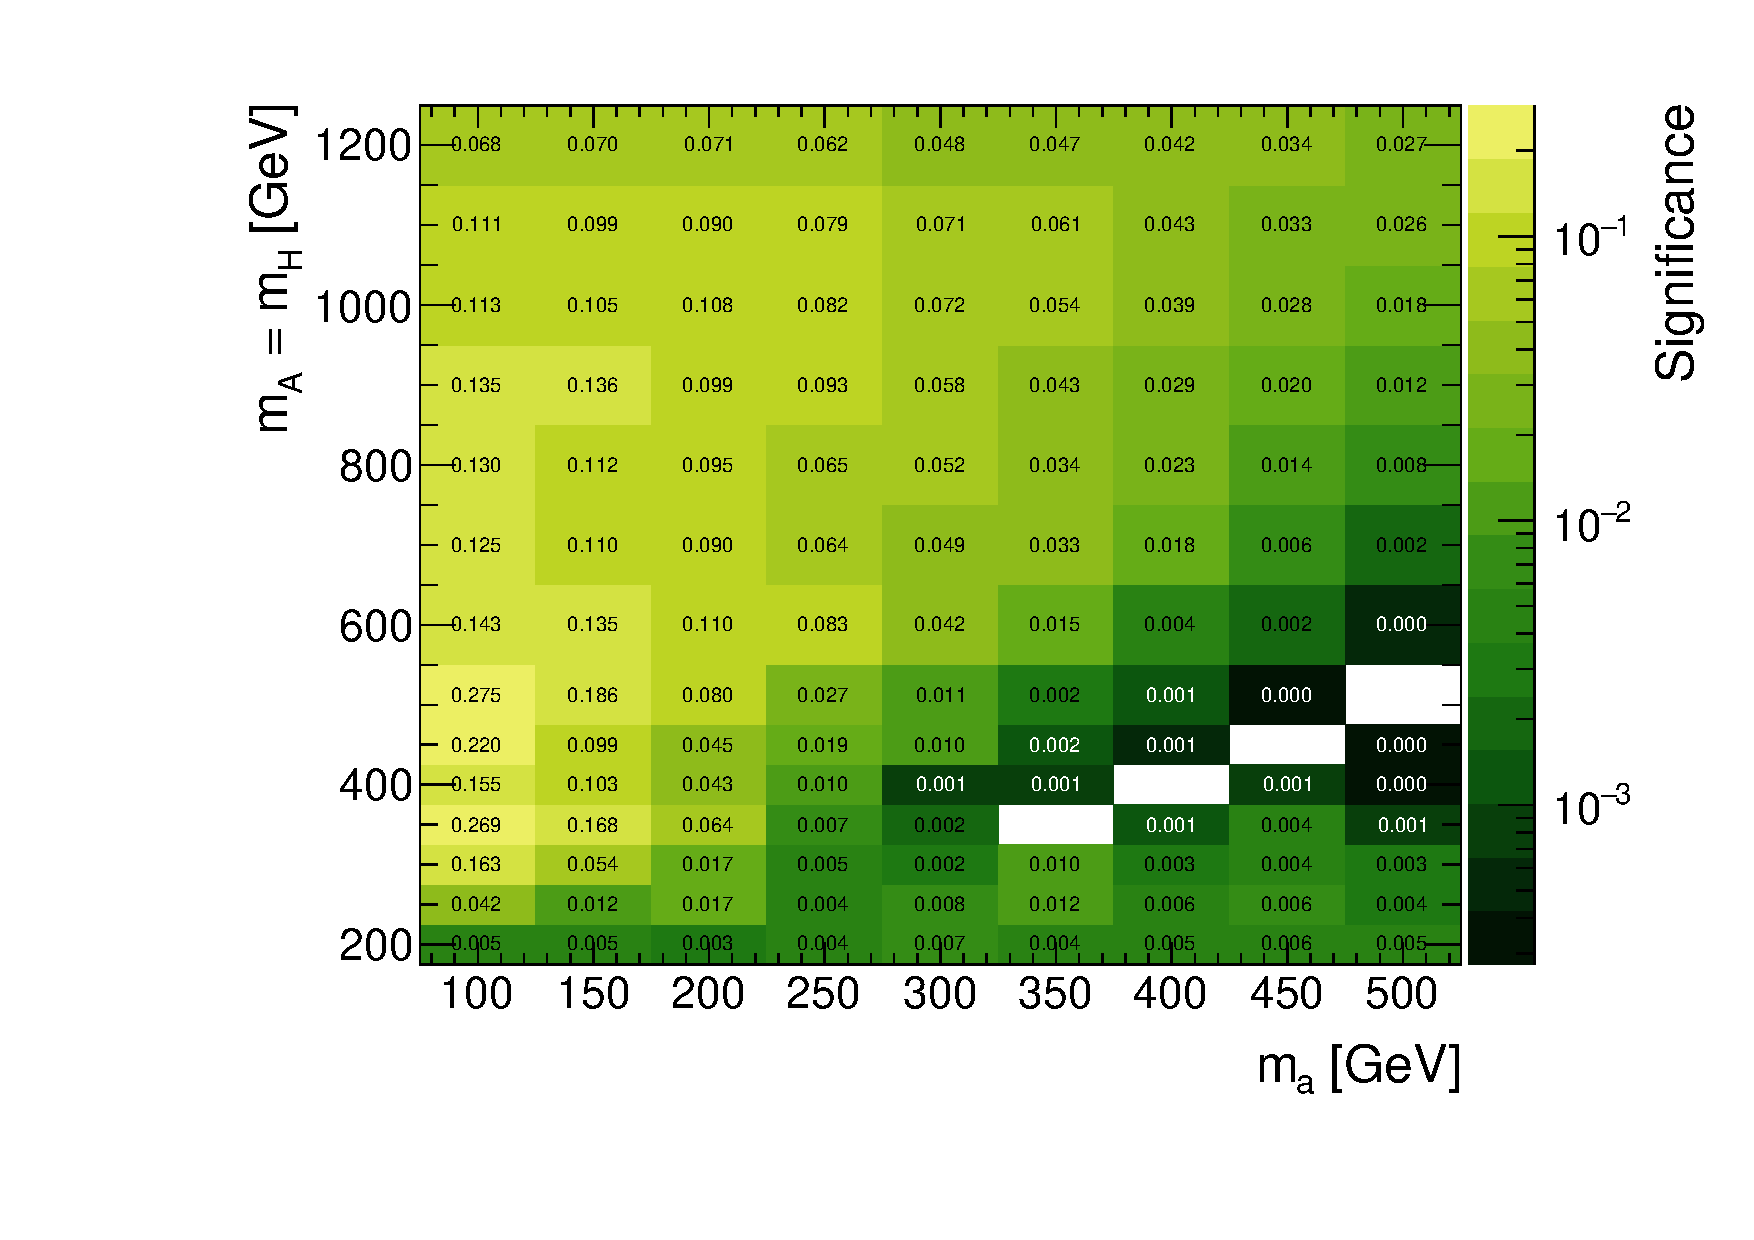
\includegraphics[width=0.45\textwidth]{texinputs/04_grid/figures/monoz/hadronic/grid_mA_ma_resl_bin100_sign_type3_bkg_uncert_0p10.pdf}
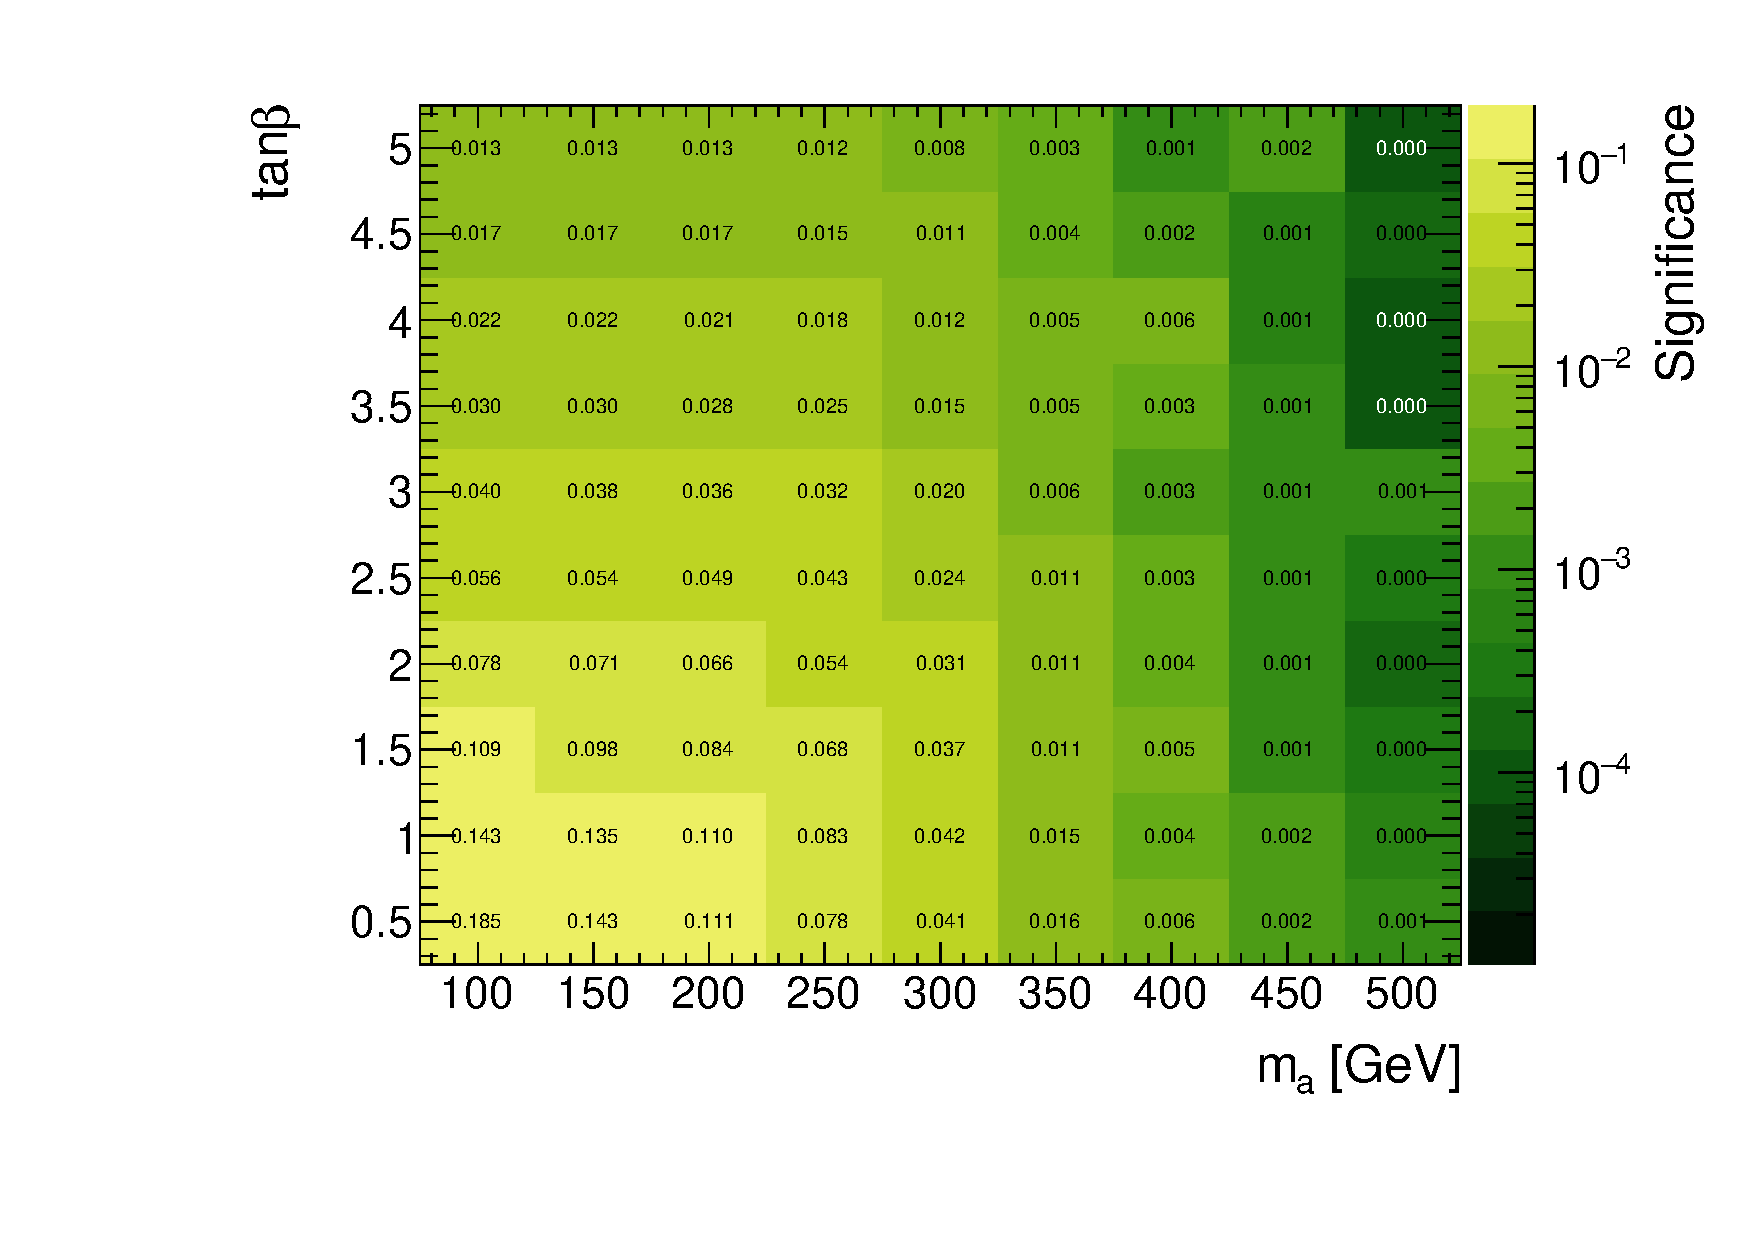
\includegraphics[width=0.45\textwidth]{texinputs/04_grid/figures/monoz/hadronic/grid_tanb_ma_resl_bin100_sign_type3_bkg_uncert_0p10.pdf}
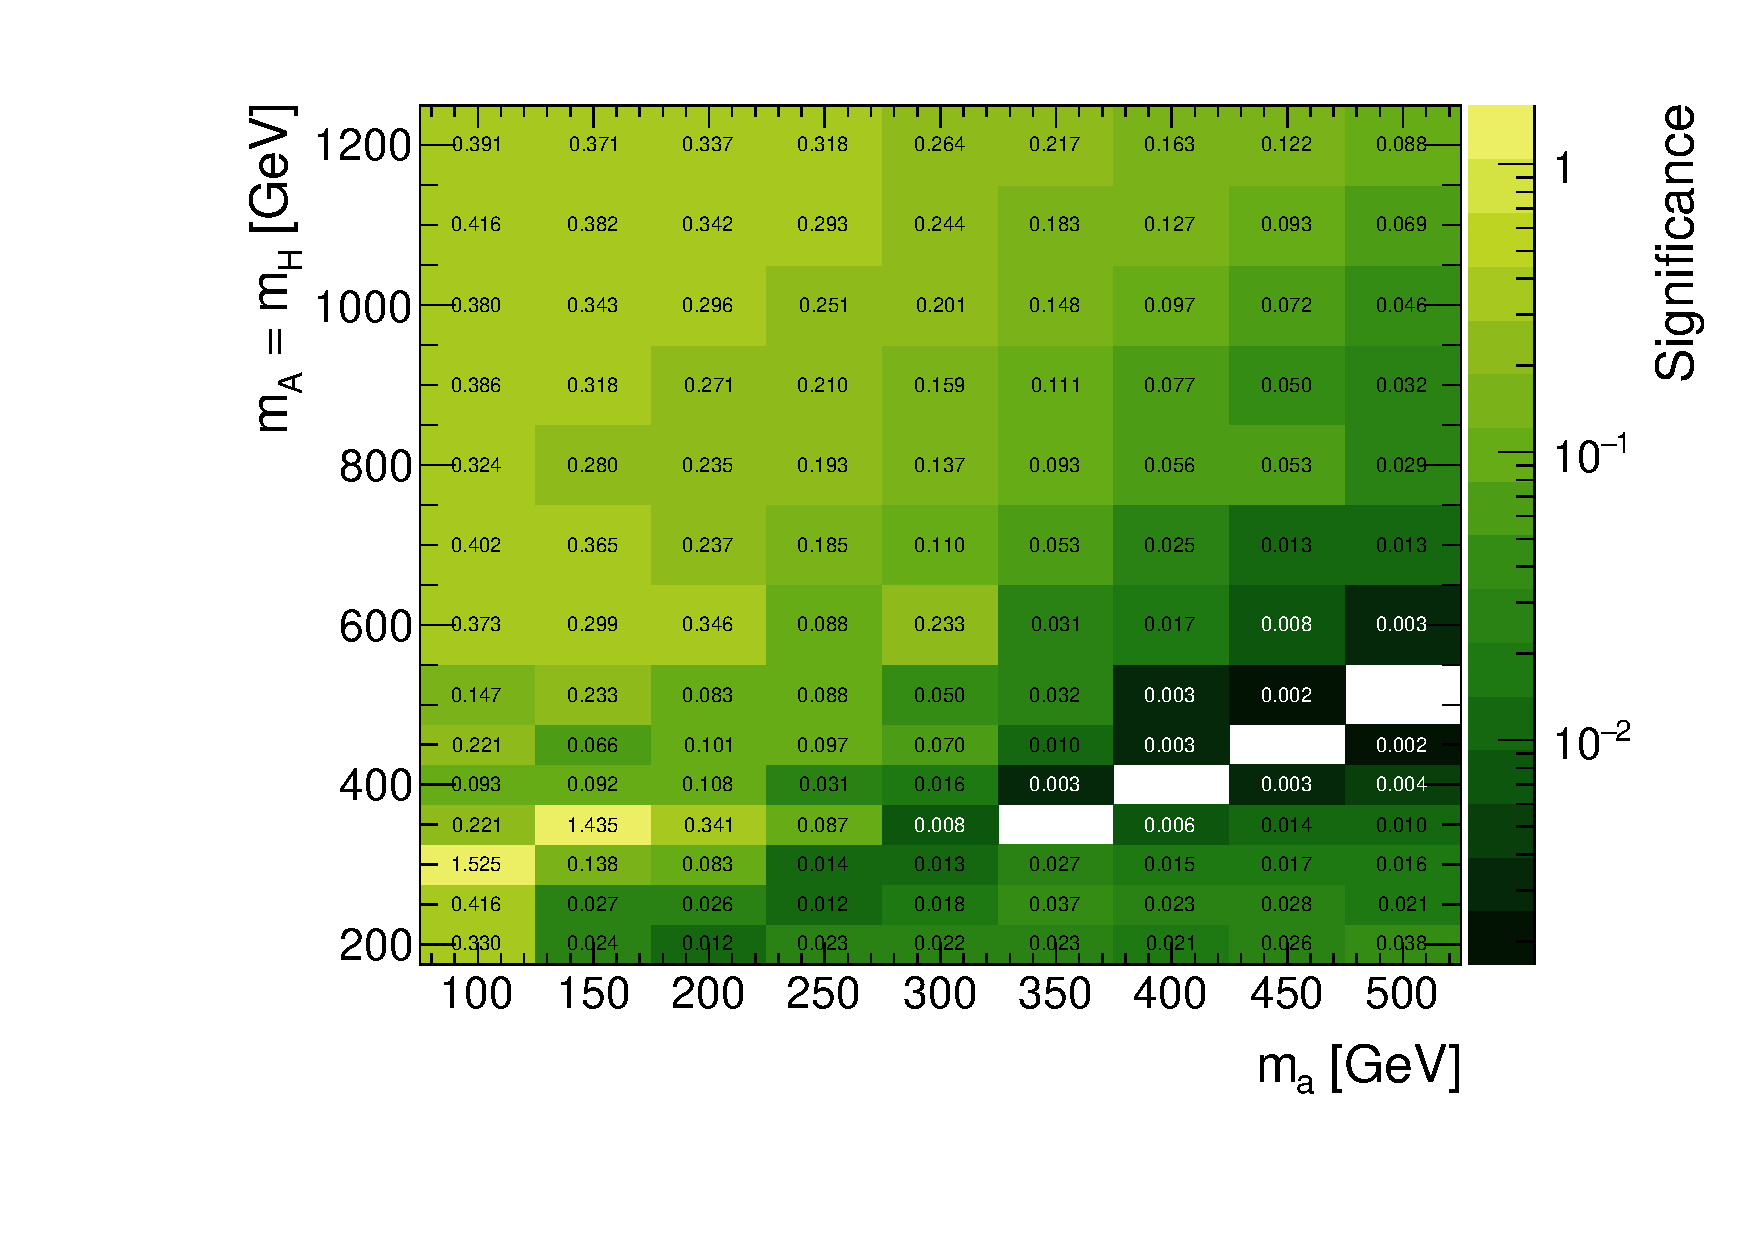
\includegraphics[width=0.45\textwidth]{texinputs/04_grid/figures/monoz/hadronic/grid_mA_ma_merged_bin100_sign_type3_bkg_uncert_0p10.pdf}
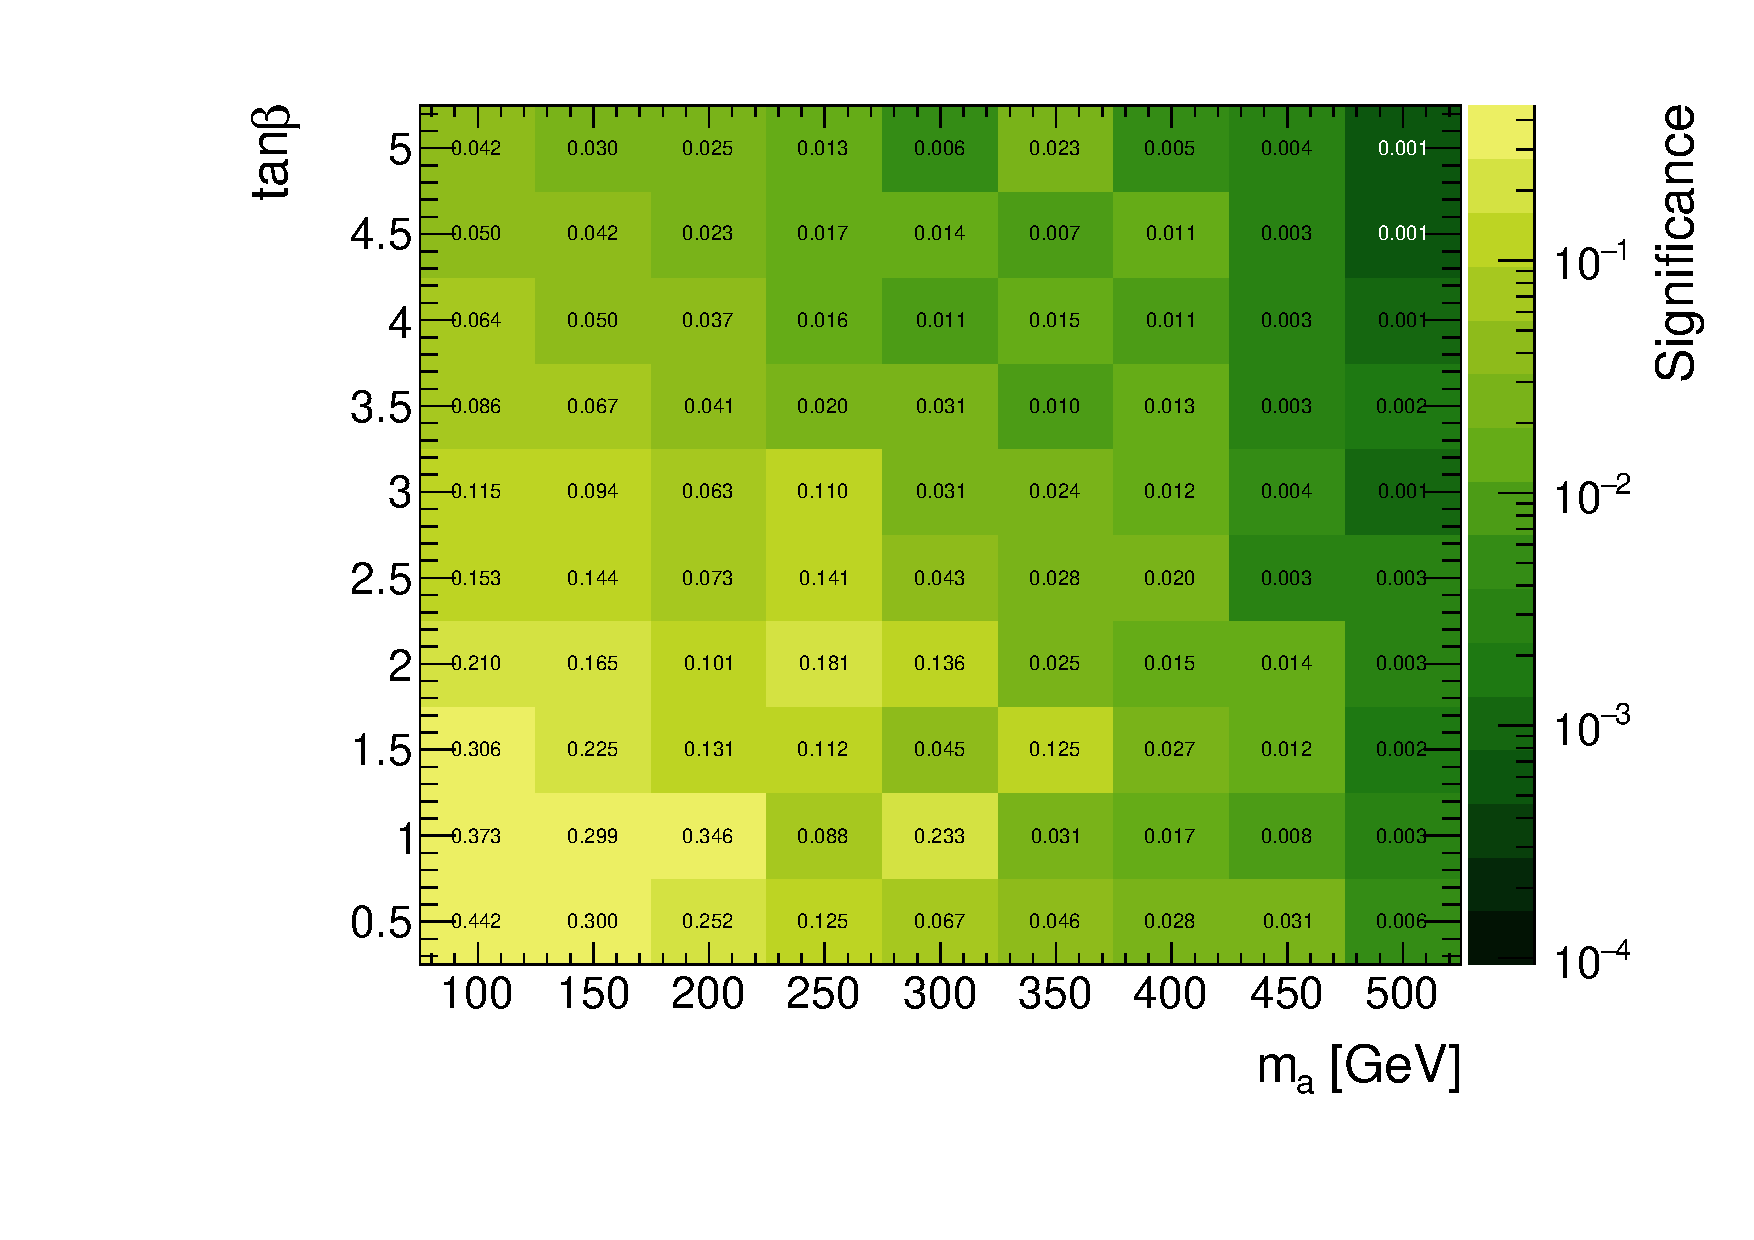
\includegraphics[width=0.45\textwidth]{texinputs/04_grid/figures/monoz/hadronic/grid_tanb_ma_merged_bin100_sign_type3_bkg_uncert_0p10.pdf}
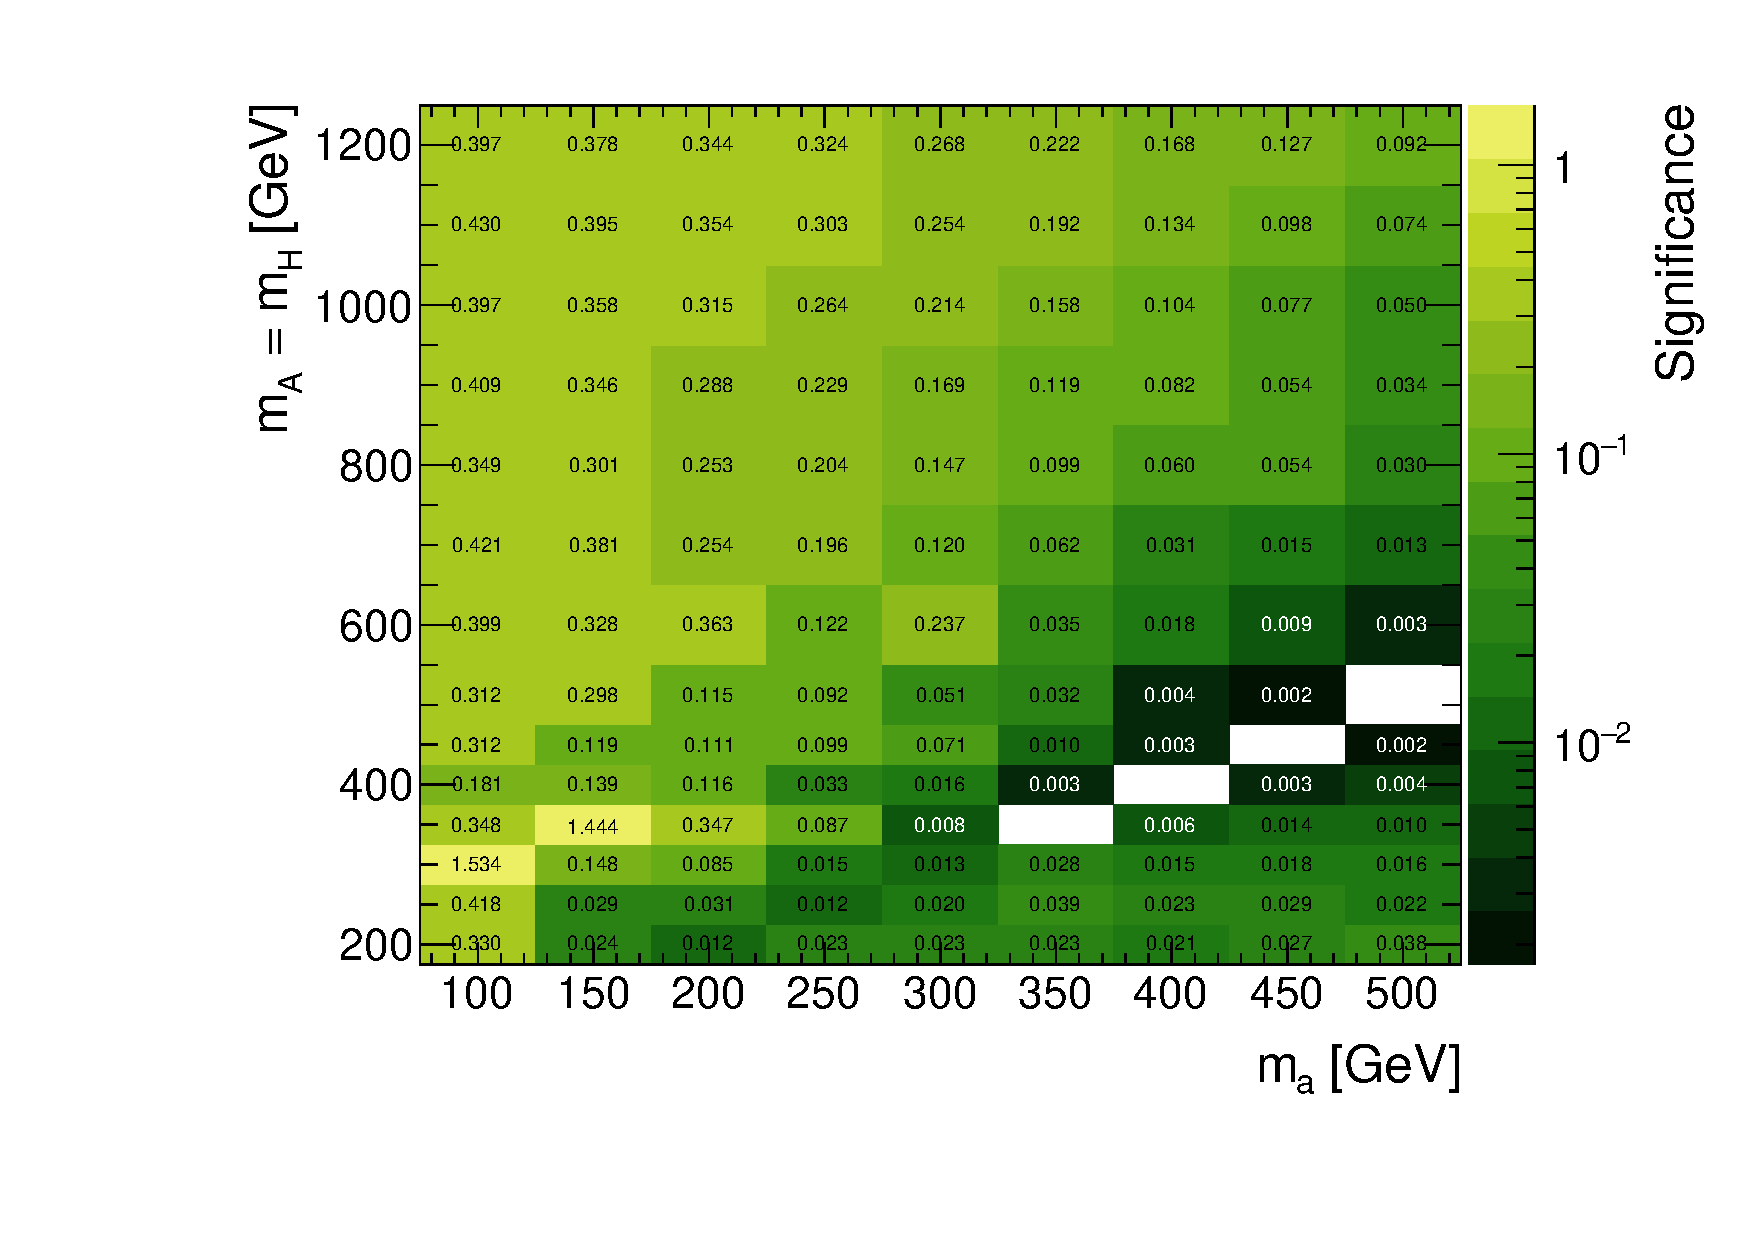
\includegraphics[width=0.45\textwidth]{texinputs/04_grid/figures/monoz/hadronic/grid_mA_ma_sum_bin100_sign_type3_bkg_uncert_0p10.pdf}
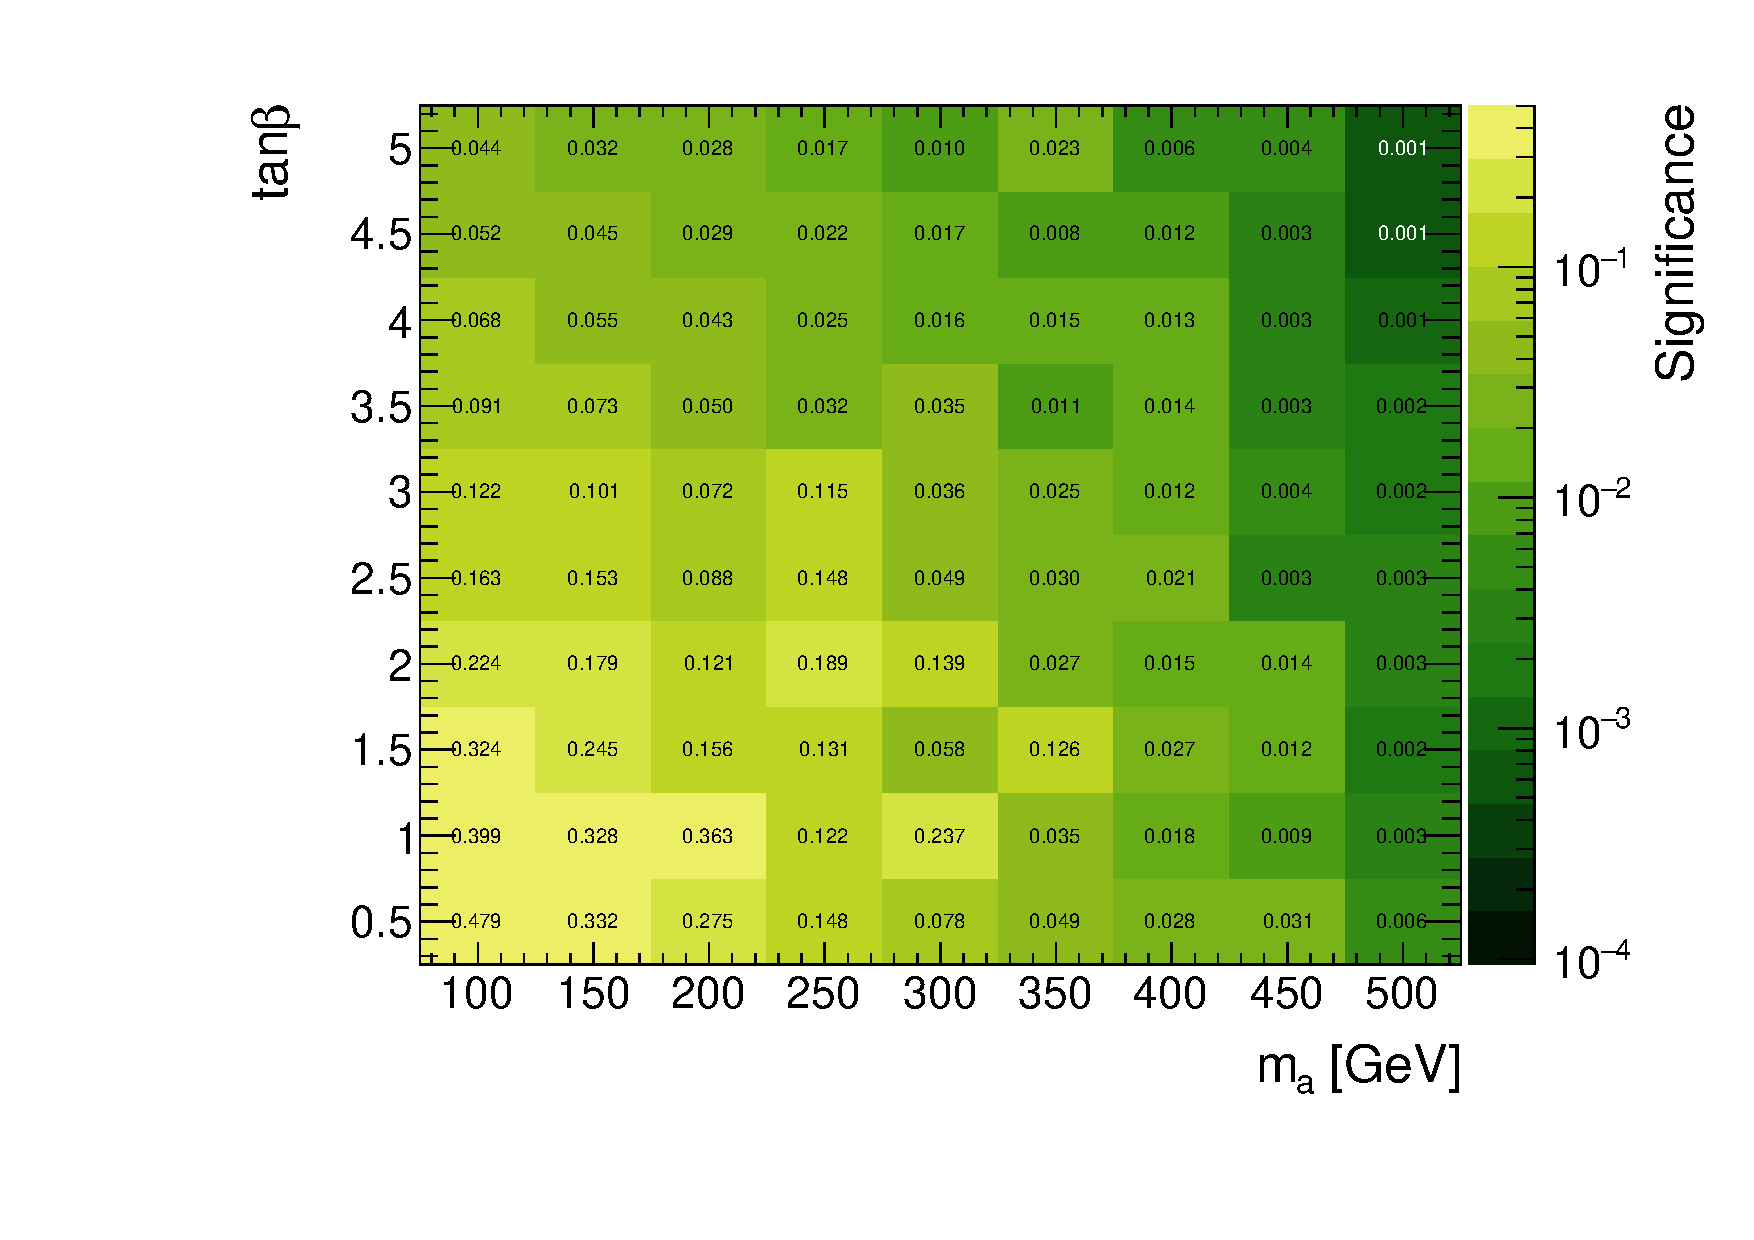
\includegraphics[width=0.45\textwidth]{texinputs/04_grid/figures/monoz/hadronic/grid_tanb_ma_sum_bin100_sign_type3_bkg_uncert_0p10.pdf}
\caption{Significance (as defined in the text) for the mono-$Z$ hadronic events 
$pp \rightarrow Z(\to q\bar{q})\chi\overline{\chi}$ in the \ma vs \mA (left) and \ma vs $\tan\beta$ (right) grids. 
Shown at the top, middle and bottom are the resolved only, boosted only and the combined resolved+boosted 
analysis, respectively.}
\label{fig:monozhad_significance_grid}
\end{figure}

The sensitivity of the resolved, boosted and the combined analysis selections to the mono-$Z$ hadronic signature 
is examined. The main background for this signature is $Z \to \nu\nu$ events in association with jets. 
The sample of $Z (\to \nu\nu)$+jets events is produced using Sherpa~2.2.1 and the matrix elements are calculated
up to 2 partons at next-to-leading order and up to 4 partons at leading order. The $Z (\to \nu\nu)$+jets events
are analyzed at particle level with the same criteria used for the signal. The number of $Z \to \nu\nu$ events 
after applying the cuts is increased by a factor 2 to account for the contribution from other backgrounds. 
This factor is chosen from the 
ATLAS dark matter search in the mono-$Z$ hadronic signature using 3.2~fb$^{-1}$ of 13~TeV data,
published in Ref.~\ref{EXOT-2015-08}. The sensitivity is defined in this study as 
%
\begin{equation}
\text{Significance} = \sqrt{\sum_{\text{bin}} Z_{\text{bin}}^2}
\label{eq:monozhad_sig}
\end{equation}
%
where the per-bin significance, $Z_{\text{bin}}$, is obtained, using asymptotic calculation of the 
Poisson likelihood ratio statistic, to be 
%
\begin{equation}
Z_{\text{bin}} = \left[ 2\left( (s+b)\ln \left[ \frac{(s+b)(b+\sigma_b^2)}{b^2+(s+b)\sigma_b^2} \right] - \frac{b^2}{\sigma_b^2} \ln \left[ 1+\frac{\sigma_b^2 s}{b(b+\sigma_b^2)} \right] \right) \right]^{1/2} 
\end{equation}
%
with the assumption of 10\% background uncertainty in each \MET bin. 
The sum in Eq.(\ref{eq:monozhad_sig}) is taken over all \MET bins after applying the final selections.
The results are shown in Fig.~\ref{fig:monozhad_significance_grid} for the resolved only, booted only and 
the combined resolved+boosted analysis selections, corresponding to the integrated luminosity of 40~fb$^{-1}$
at $\sqrt{s} = 13$~TeV. The significance depends strongly on the assumption of background uncertainty 
since a large number of background events remain in this simple analysis with a minimum set of selection criteria.
More realistic analysis performed in LHC experiments is expected to improve the sensitivity.

